%! Tex program = xelatex   
\documentclass{article}
\usepackage{graphicx,subfig}
\usepackage[left=2cm, right=2cm, lines=45, top=0.8in, bottom=0.7in]{geometry}
\usepackage{xeCJK}
\usepackage{amsmath}
\usepackage{booktabs} %表格
\usepackage{tikz}
\usepackage{graphics}
\usepackage{xcolor} 
\usepackage{tikz} 
\usepackage{svg}
\usetikzlibrary{arrows,shapes,chains}
\setmainfont{Times New Roman}
\setCJKmainfont{Songti SC}
\setCJKfamilyfont{song}{Songti SC}
\renewcommand{\baselinestretch}{1.5} %行间距
%-----------------------伪代码------------------
\usepackage{algorithm}  
\usepackage{algorithmicx}  
\usepackage{algpseudocode}  
\floatname{algorithm}{Algorithm}  
\renewcommand{\algorithmicrequire}{\textbf{Input:}}  
\renewcommand{\algorithmicensure}{\textbf{Output:}} 
\usepackage{lipsum}  
\makeatletter
\newenvironment{breakablealgorithm}
  {% \begin{breakablealgorithm}
  \begin{center}
     \refstepcounter{algorithm}% New algorithm
     \hrule height.8pt depth0pt \kern2pt% \@fs@pre for \@fs@ruled
     \renewcommand{\caption}[2][\relax]{% Make a new \caption
      {\raggedright\textbf{\ALG@name~\thealgorithm} ##2\par}%
      \ifx\relax##1\relax % #1 is \relax
         \addcontentsline{loa}{algorithm}{\protect\numberline{\thealgorithm}##2}%
      \else % #1 is not \relax
         \addcontentsline{loa}{algorithm}{\protect\numberline{\thealgorithm}##1}%
      \fi
      \kern2pt\hrule\kern2pt
     }
  }{% \end{breakablealgorithm}
     \kern2pt\hrule\relax% \@fs@post for \@fs@ruled
  \end{center}
  }
\makeatother
%------------------------代码-------------------
\usepackage{xcolor} 
\usepackage{listings} 
\usepackage{fontspec}
\newfontfamily\menlo{Menlo}
\setmonofont[Mapping={}]{Monaco} 
\definecolor{mygreen}{rgb}{0,0.6,0}
\definecolor{mygray}{rgb}{0.5,0.5,0.5}
\definecolor{mymauve}{rgb}{0.58,0,0.82}
\lstset{ %
backgroundcolor=\color{white},   % choose the background color
basicstyle=\footnotesize\ttfamily,        % size of fonts used for the code
columns=fullflexible,
breaklines=true,                 % automatic line breaking only at whitespace
captionpos=b,                    % sets the caption-position to bottom
tabsize=4,
commentstyle=\color{mygreen},    % comment style
escapeinside={\%*}{*)},          % if you want to add LaTeX within your code
keywordstyle=\color{blue},       % keyword style
stringstyle=\color{mymauve}\ttfamily,     % string literal style
frame=single,
rulesepcolor=\color{red!20!green!20!blue!20},
numbers=left,
 numberstyle=\tiny\menlo
identifierstyle=\color{red},
% language=c++,
}
\begin{document}
\title{核酸检测登记系统}
\author{朱浩泽 1911530 \ \ \ 何坤彬 1911417}
\maketitle
\section{软件需求和设计}
\large
\subsection{需求背景}
2020年伊始,一场突如其来的新型冠状病毒肺炎疫情,在春节期间突袭神州大地,面对困难,举国上下团结一心,共同投入到抗击疫情的工作中。在党中央坚强领导下,中国人民风雨同舟、众志成城,发扬一方有难、八方支援精神,构筑起疫情防控的坚固防线。广大医务人员白衣为甲、逆行出征,为保障人民的健康,进行了一轮又一轮的健康监测。而这些检测结果的数据量是庞大的,这就需要我们对海量的信息进行有效的组织管理,来确保信息的准确性和完整性。于是,我们计划开发一款核酸检测登记系统。
\subsection{系统设计思路}
\ \ \ \ \ 在拥有需求之后,我们可以对我们的系统进行设计。首先,核酸登记系统需要识别被登记人,而如果用人名作为登记人员的信息,可能会有很多重名的人员导致信息混乱。所以我们需要选取每个人都具有的且为独一无二的表示方式。在现如今的社会,每个人都拥有着自己的身份证号,且是一人一号,具有问一下。由此可见身份证号可以很好的承载着我们的需求,故选取身份证号作为登记人员的身份标识,配合被测人员的姓名进行辅助。

接下来便是,当我们获得了人员的信息后,需要存储其核酸检测状态,所以需要存储人员的检测情况(阴性/阳性)。在检测后,我们也要给被测人员一个检测情况的反应,并在必要时(万一呈现阳性时)可以找到被测人员,所以我们要记录被测人员的手机号以便进行联系和反馈,并登记被检测人员的住址进行潜在的流行病学调查。由于疫情发展瞬息万变,一个人可能会测多次核酸,所以我们还要记录其检测时间,以区分不同批次检测结果。而且,不同人群的身体反应可能也是不一样的,所以我们还要记录人员的年龄信息。所以我们。这里我们选择了一个简单的数据库,其中包含了人员的身份证号、姓名、检测状态(阴性/阳性)、检测时间、检测结果(阴性/阳性)。

当然,为了加快信息录入的速度,我们允许多人对信息进行登录。同时又避免信息的混乱和保证信息的安全性,我们采取了注册制度。用户需要先进行注册,然后医护人员才可以为用户的核酸检测数据进行上传和更改,由于核酸检测只有最近的结果是有说服性的,所以我们每次登记时只相当于更改被登记人的最后一次见的时间和检测记录。

我们采用java框架配合mysql数据库进行系统设计。

\section{用户界面交互展示}
\subsection{登录}
\begin{center}
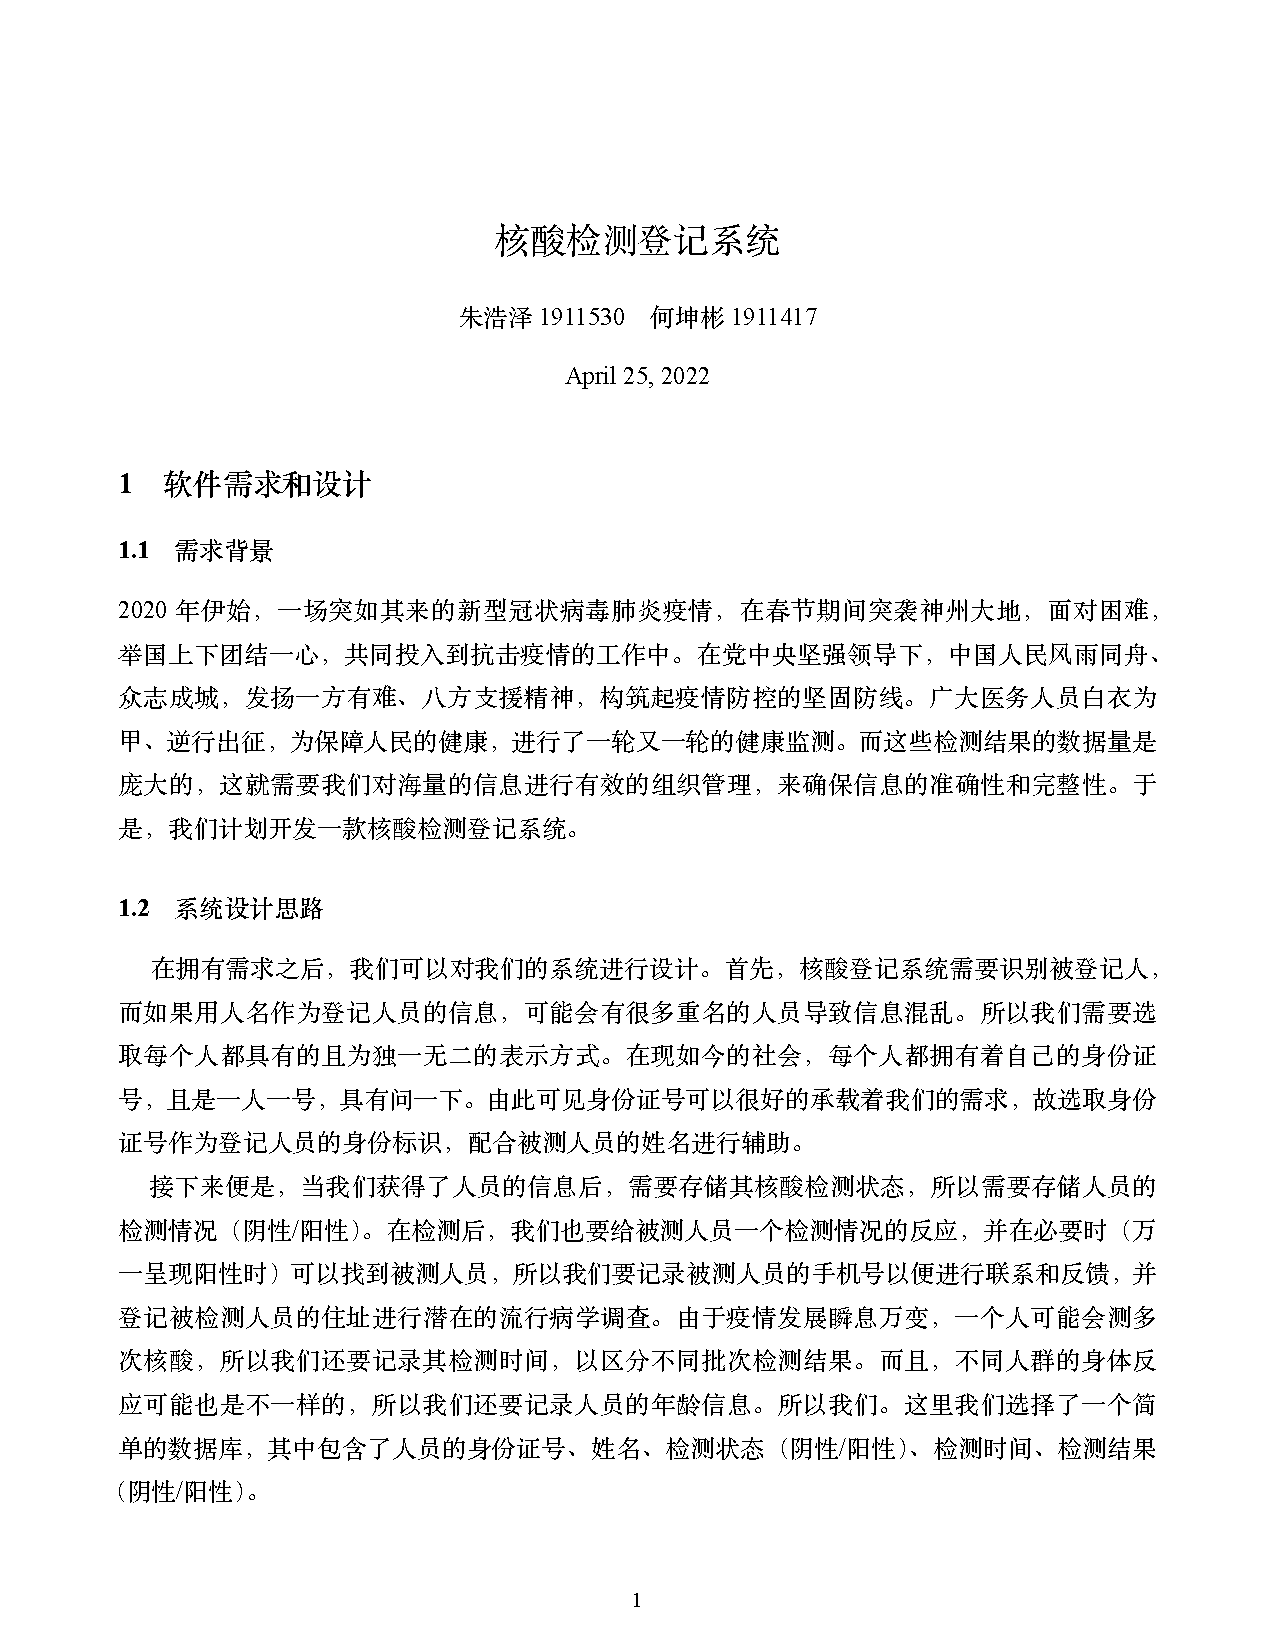
\includegraphics[width=0.5\textwidth]{图片/1}
\includegraphics*[width=0.5\textwidth]{图片/2}
\end{center}
\subsection{登录后的界面}
\begin{center}
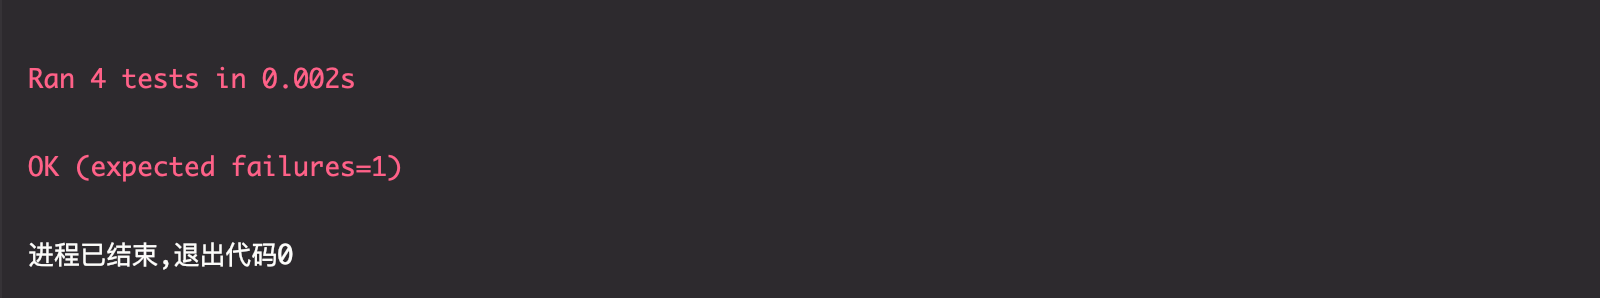
\includegraphics[width=0.5\textwidth]{图片/3}
\end{center}
\subsection{用户注册}
\begin{center}
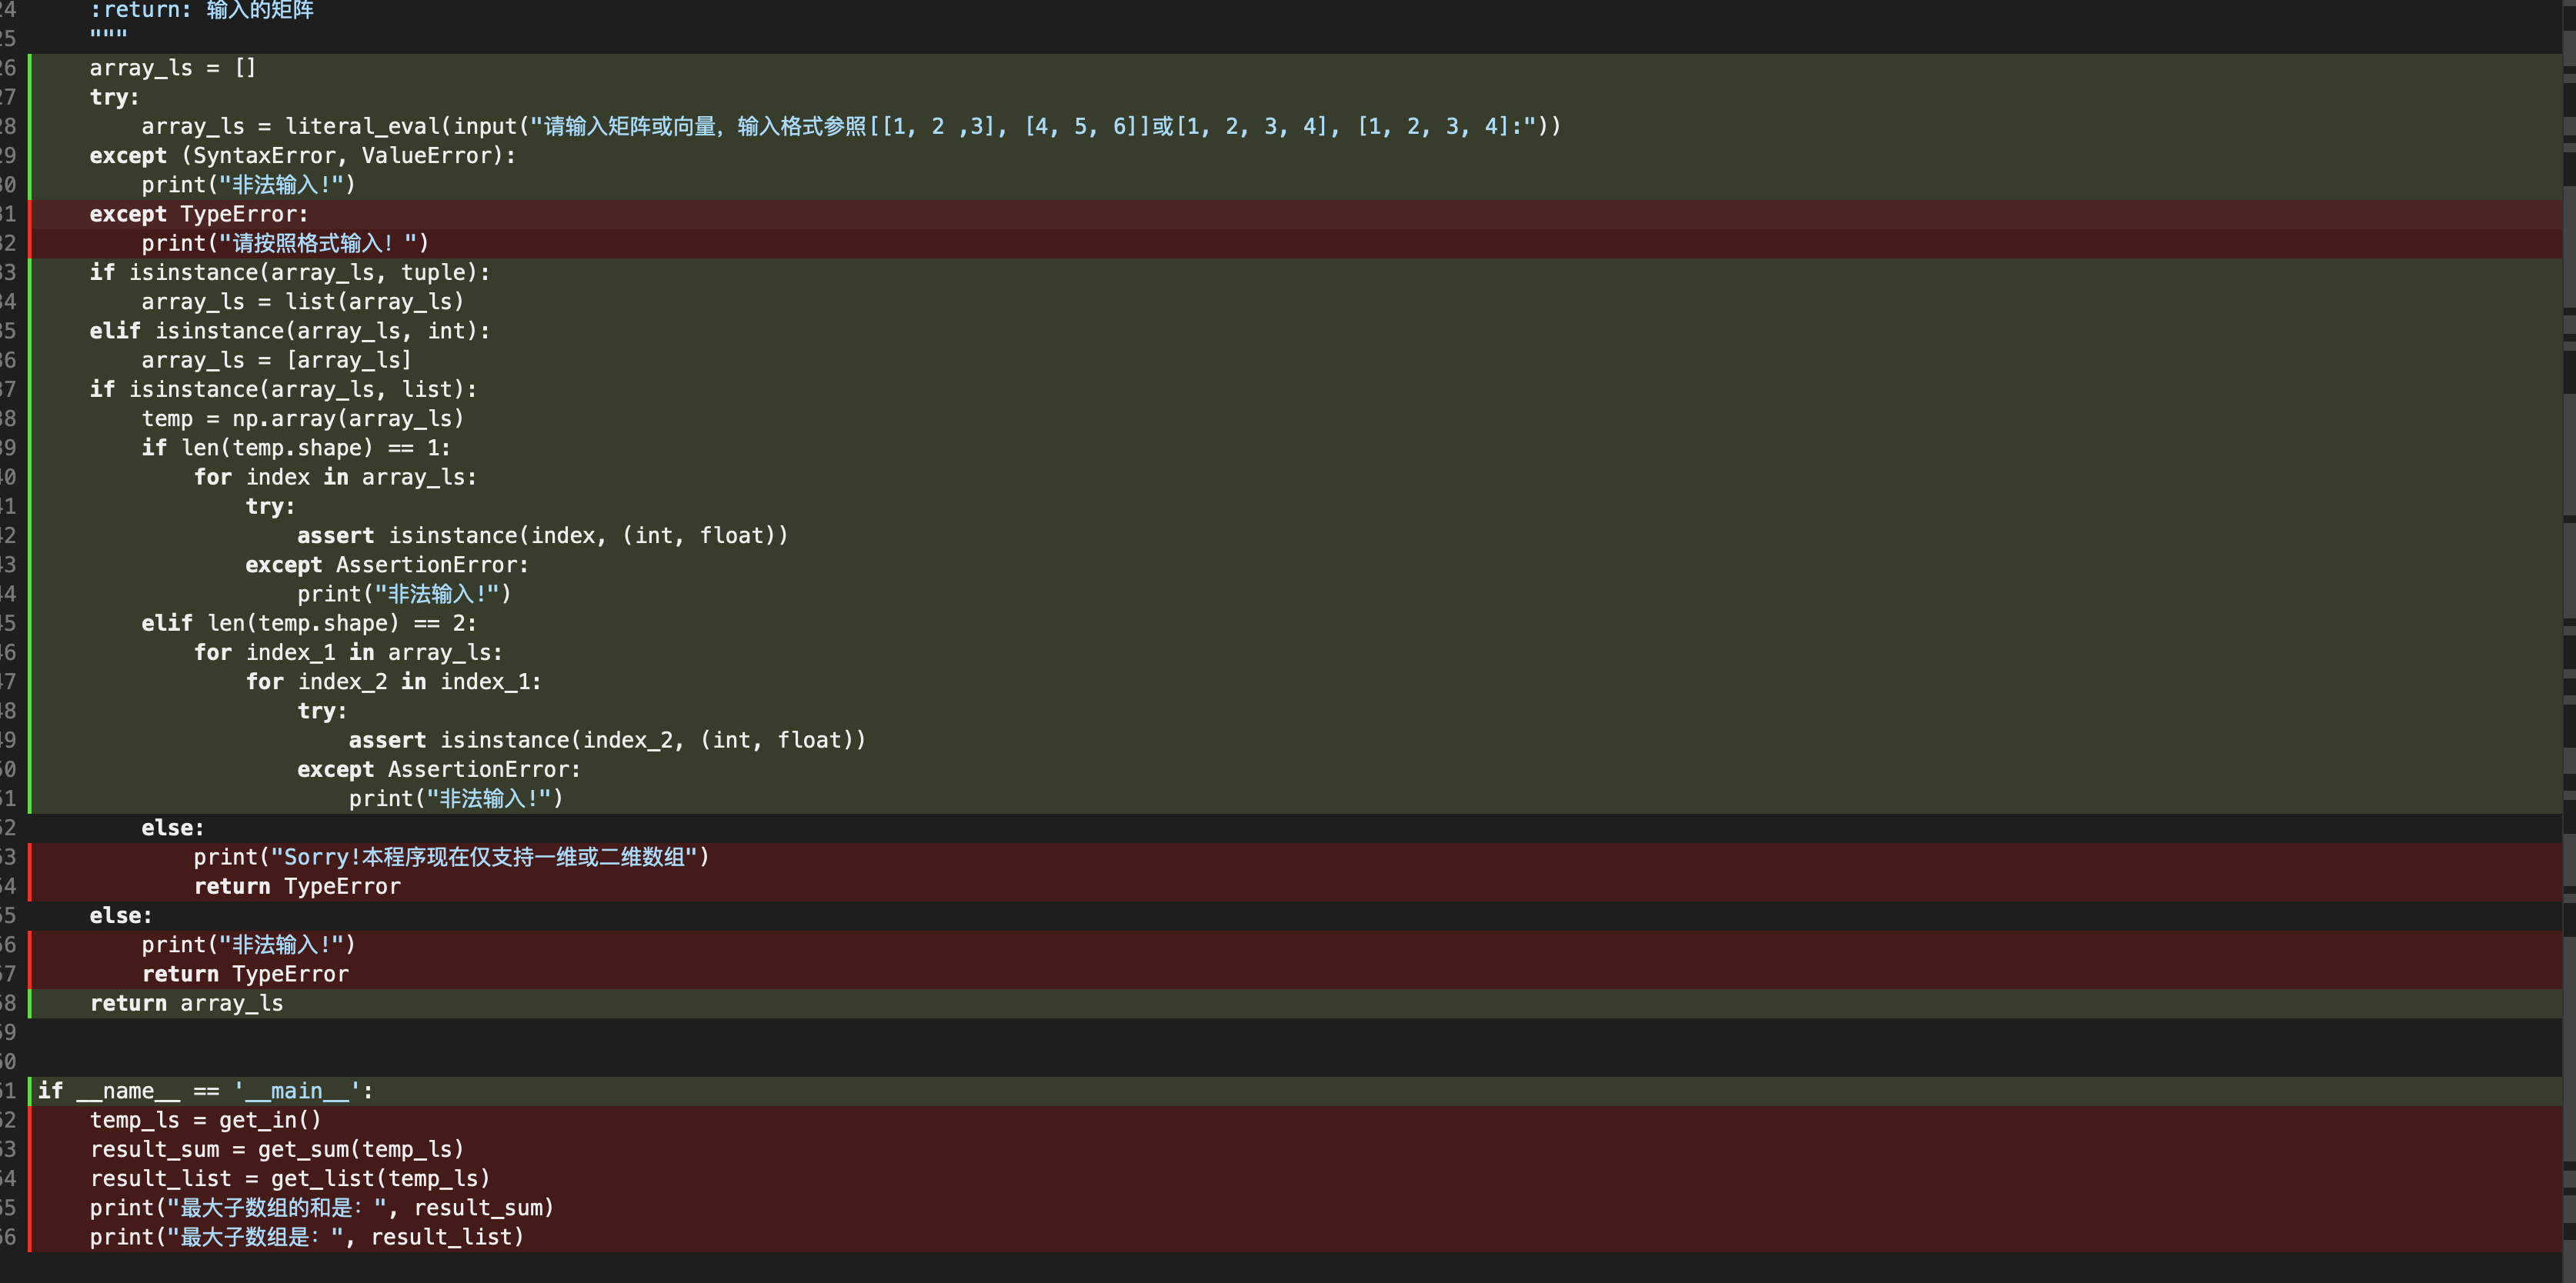
\includegraphics[width=0.5\textwidth]{图片/4}
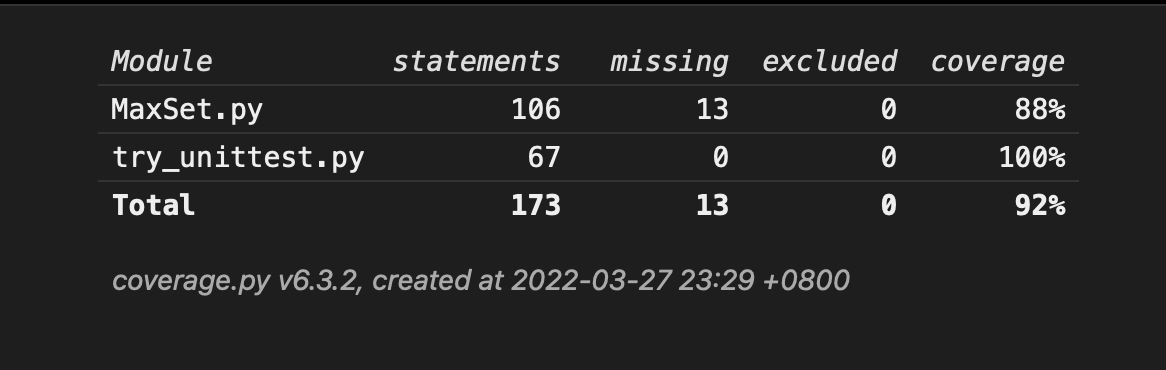
\includegraphics[width=0.5\textwidth]{图片/5}
\includegraphics[width=0.5\textwidth]{图片/6}
\end{center}
注册成功后刷新便可以看到人员信息
\begin{center}
\includegraphics[width=0.5\textwidth]{图片/7}
\includegraphics[width=0.5\textwidth]{图片/8}
\end{center}
\subsection{查询}
\begin{center}
\includegraphics[width=0.5\textwidth]{图片/9}
\includegraphics[width=0.5\textwidth]{图片/10}
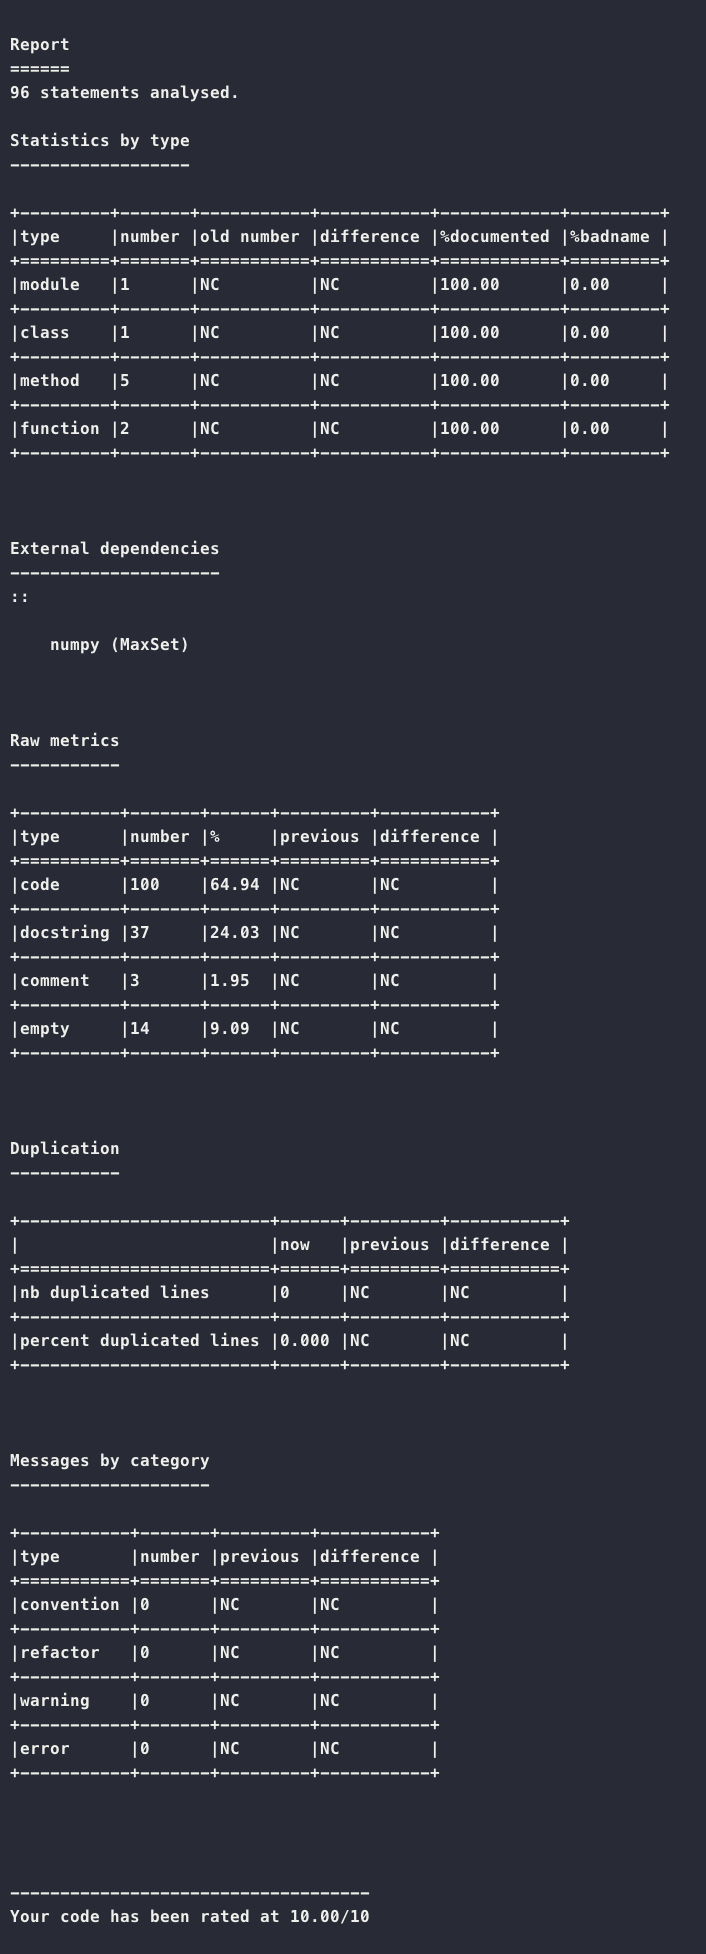
\includegraphics[width=0.5\textwidth]{图片/11}
\includegraphics[width=0.5\textwidth]{图片/12}
\includegraphics[width=0.5\textwidth]{图片/13}
\end{center}
\subsection{登记检测结果}
\begin{center}
\includegraphics[width=0.5\textwidth]{图片/14}
\includegraphics[width=0.5\textwidth]{图片/16}
\includegraphics[width=0.5\textwidth]{图片/17}
\includegraphics[width=0.5\textwidth]{图片/18}
\end{center}

刷新后可以看到新登记的检测结果

\begin{center}
\includegraphics[width=0.5\textwidth]{图片/19}
\includegraphics[width=0.5\textwidth]{图片/20}
\includegraphics[width=0.5\textwidth]{图片/21}
\includegraphics[width=0.5\textwidth]{图片/22}
\end{center}
\section{角色轮换安排}
我们的角色轮换较为明确,在编写数据库和设计数据库这一部分时,由何坤彬充当领航员,朱浩泽充当驾驶员;在进行java部分的可视化操作时,由朱浩泽充当领航员,何坤彬充当驾驶员。
\section{代码复审及讨论改进的过程}
\ \ \ \ \ \ 在最初,我们设计的mysql表非常简单,只有一个检测结果表(身份证号,姓名,检测结果)和一个用户表(用户名,密码),但此时领航员立刻指出,这样无法将用户表和检测结果表关联起来,所以增加了用户id这一特征将两张表中的内容进行关联。


\section{双人合作的工作照片}
\section{对方编程习惯总结和性格评价}
\section{心得体会}
\end{document}
